\documentclass{article}
\usepackage{minted}

% \usepackage{graphics}      % for EPS, load graphicx instead 
\usepackage{graphicx} 

% if you need to pass options to natbib, use, e.g.:
    \PassOptionsToPackage{square,numbers}{natbib}
% before loading neurips_2020
% to avoid loading the natbib package, add option nonatbib:
    %  \usepackage[nonatbib]{neurips_2020}

% ready for submission
% \usepackage{neurips_2020}
% \usepackage{biblatex}
% \bibliography{bibliography}
% \addbibresource{bibliography.bib}
% to compile a preprint version, e.g., for submission to arXiv, add add the
% [preprint] option:
    % \usepackage[preprint]{neurips_2020}
% \bibliography{bibliography}

% to compile a camera-ready version, add the [final] option, e.g.:
    \usepackage[final]{neurips_2020} %for some reason gotta uncomment this line to show the authors (otherwise it looks as anonymous)
\usepackage[nottoc]{tocbibind}
\bibliographystyle{abbrvnat} %necessary for the bibligraphy to show


\usepackage[utf8]{inputenc} % allow utf-8 input
\usepackage[T1]{fontenc}    % use 8-bit T1 fonts
\usepackage{hyperref}       % hyperlinks
\usepackage{url}            % simple URL typesetting
\usepackage{booktabs}       % professional-quality tables
\usepackage{amsfonts}       % blackboard math symbols
\usepackage{nicefrac}       % compact symbols for 1/2, etc.
\usepackage{microtype}      % microtypography

\title{Human Cognition Based Word Segmentation Models}

% The \author macro works with any number of authors. There are two commands
% used to separate the names and addresses of multiple authors: \And and \AND.
%
% Using \And between authors leaves it to LaTeX to determine where to break the
% lines. Using \AND forces a line break at that point. So, if LaTeX puts 3 of 4
% authors names on the first line, and the last on the second line, try using
% \AND instead of \And before the third author name.

\author{
  Shinjini Ghosh \\
  Department of Electrical Engineering and Computer Science, MIT \\
  \texttt{shinghos@mit.edu} \\
  % examples of more authors
  \And
  Raul Alcantara \\
  Department of Electrical Engineering and Computer Science, MIT \\
  \texttt{ralcanta@mit.edu} \\
}

\begin{document}

\maketitle

\begin{abstract}
    Segmentation of words from free speech or unsegmented text is an almost universally prevalent human skill. In this article, we build, implement and test three computational models of word segmentation based on human cognition---a probabilistic context-free grammar model, a probabilistic \texttt{n}-gram model with dynamic programming, and a statistical Viterbi algorithm based approach. We also investigate how they perform in comparison with human cognition experiments in similar conditions.
%   The abstract paragraph should be indented \nicefrac{1}{2}~inch (3~picas) on
%   both the left- and right-hand margins. Use 10~point type, with a vertical
%   spacing (leading) of 11~points.  The word \textbf{Abstract} must be centered,
%   bold, and in point size 12. Two line spaces precede the abstract. The abstract
%   must be limited to one paragraph.
\end{abstract}

\section{Introduction}

Word segmentation is the process of determining the word boundaries in free-flowing speech or non-segmented text. Language learners of all ages are able to naturally demarcate word boundaries from continuous speech, even without appreciable pauses or other linguistic cues (as mentioned in \citet{Saffran1996}). So how is that human cognition allows for word segmentation within such poverty of stimulus? And is there a way we can capture the same computationally for our use in language modeling and beyond?

There have been several attempts and ongoing work for finding different algorithms that will efficiently and accurately segment any given sentence, text, or speech, either in English or in another language. One of the pioneers in this was Saffran et al., who analyzed how children performed this task from a very young age. After her study, different approaches were taken, both in the classical statistics (\citet{Brent}, \citet{Venkataraman}) and Bayesian realms (\citet{GOLDWATER200921}). In this paper, we try to develop on and implement some of these methods, and analyze their performance on the segmentation task, given different unsegmented corpora, especially in relation with human judgements.

\section{Motivation}
% We are interested in projects at the intersection of cognitive science and linguistics. 
We believe that
current state-of-the-art language models, which fail on natural language understanding and inference tasks, could benefit with human-inspired augmentations and that an improved word segmentation algorithm would further the current NLP frontiers in the capabilities of neural and non-neural language models, especially because most models currently in place crucially reply on segmenting words correctly. We wish to distil the knowledge gained from our understanding of human cognition into computational models and human-like intelligent systems.

% Specifically, we want to answer the question ``Can we apply intuitions about human cognition to investigate and improve word segmentation beyond the performance of current quantitative models?" in this project. 

% We wish to explore multiple avenues for word segmentation, including designing a useful metric and either collecting human judgments on various segmentations of words or looking at existing datasets, and eventually trying to build an algorithm inspired by human cognitive processes. We also want to look at, reimplement and possibly tweak current state-of-the-art algorithms and investigate into how ours differs from them. This also necessitates the development of a framework for comparing word segmentation algorithms: how do we know if a segmentation is ``correct" or more ``accurate" or considered more ``natural" by humans? Eventually, we aim to have a comparison across existing and new word segmentation algorithms, which can help highlight the contributions induced by human judgements.

% \section{Background Research}

\section{Saffran Revisited, Computationally}
% \vspace{-6mm}
\citet{Saffran1996}'s groundbreaking paper delves into statistical learning by 8-month-old infants, and aims to probe one of the very basic human cognitive tasks, a fundamental task accomplished by almost every child in the world---segmentation of words from fluent speech. The authors state that `successful' word segmentation by the infants, based on only 2 minutes of speech exposure, suggests that they have access to a powerful mechanism for computing the statistical properties of language input. This is a very important observation in building computational models of cognition regarding word segmentation, especially when coupled with the fact that there exists complex and widely varying acoustic structure of speech in different languages and hence, there is no invariant acoustic cue to word boundaries present in all languages.

In the class goal of `reverse-engineering the human mind', Saffran et al.'s observations are crucial as we set out to use knowledge of how human intelligence works in order to build more human-like intelligence systems [Class Slides, Lecture 1]. As outlined in \citet{Goodman2014ConceptsIA}, \citet{Goodmand&Tenenbaum2016}, \citet{Tenenbaum2012} and multiple other papers, the probabilistic language of thought hypothesis believes that concepts have a language-like compositionality and encode probabilistic knowledge, thereupon relying on Bayesian inference for production. We also look at how \citet{GOLDWATER200921} approach the word segmentation problem probabilistically, relying on word context. Extending from the word learning concepts of Lectures 1 and 5, and the categorization concepts of Lectures 22 and 23, we try to revisit Saffran et al.'s experiment, this time computationally.
% \vspace{-8mm}
\subsection{Modeling with Probabilistic Context Free Grammars (PCFGs)}
% \vspace{-4mm}
We use a Probabilistic Context Free Grammar to computationally explore Saffran et al.'s experiment, and see how our probabilistic model performs in comparison with human infants. In class, we saw how PCFGs perform Bayesian inference for the sentence `I shot an elephant in my pajamas', and what the various valid parses for this sentence are. In \citet{Johnson2007BayesianIF}, Bayesian inference for PCFGs via MCMC is used for morphology. We adapt a similar ideology to word segmentation as follows, where a PCFG captures word segmentation as inference.

\subsection{PCFG Setup}
We modify the usual PCFG setup as follows. Instead of having an input sentence, we have an input speech stream, segmented into syllables. We assume that the smallest part of speech that infants can discern without external knowledge is syllables (Saffran et al. also take tri-syllabic words and look at probability transitions between word boundaries in infants), and our concern is how they break this syllable stream into words. We then segment the speech stream aka `Sentence' into words, which further break into more words or a single word, which break into syllable(s).

Our sample PCFG thus looks as follows.
\vspace{-3mm}
\begin{minted}
[
frame=lines,
framesep=2mm,
baselinestretch=1.2,
% fontsize=\footnotesize,
linenos
]
{python}
    """ 
    Sentence -> Words [1.0]
    Words -> Word Words [0.8] | Word [0.2]
    Word -> Syllables [1.0]
    Syllables -> Syllable Syllables [0.8] | Syllable [0.2]
    Syllable -> 'tu' [0.083]
    Syllable -> 'pi' [0.168]
    Syllable -> 'ro' [0.083]
    Syllable -> 'go' [0.083]
    Syllable -> 'la' [0.168]
    Syllable -> 'bu' [0.083]
    Syllable -> 'da' [0.083]
    Syllable -> 'ko' [0.083]
    Syllable -> 'ti' [0.083]
    Syllable -> 'du' [0.083] 
    """

\end{minted}

Just like Saffran et al., we generate speech stream by randomly concatenating words from the input vocabulary (of 2 minutes = 180 words). The syllable probabilities are then inferred from the speech stream, and the word/syllable break probabilities are a parameter that we tweak and see the results with. We then investigate the various word parses (and corresponding) that these PCFGs give us, as well as the probabilities of those parses. A sample parse tree with high probability is shown in Fig~\ref{fig:figure1}---it shows us how given a stream of syllables, our PCFG breaks down the input `da ro pi go la tu' into two words `daropi' and `golatu'. This is one of the ``hard" input examples for the vocabulary consisting of the words ``pigola", ``golatu", and ``daropi", because the `part-word' ``pigola" spanned the boundary between `daropi\#golatu'. Below that, we have another parse tree in Fig~\ref{fig:figure2}---one with a low probability assigned by the parser, and clearly not adequate. We hypothesize that humans have access to such computing mechanism, and select a high probability parse tree to use in their daily lives.

% \begin{figure}[h]
%     \centering
%     \includegraphics[scale=0.8]{sample_tree.png}
%     \caption{Sample Parse Tree}
%     \label{fig:sample_tree}
% \end{figure}

% \includegraphics[scale=0.8]{sample_tree.png}
\begin{figure}[h!]
  \centering
  \includegraphics[width=\columnwidth]{figures/sample_tree.png}
  \caption{Sample Parse Tree with High Probability}~\label{fig:figure1}
\end{figure}

\begin{figure}[h!]
  \centering
  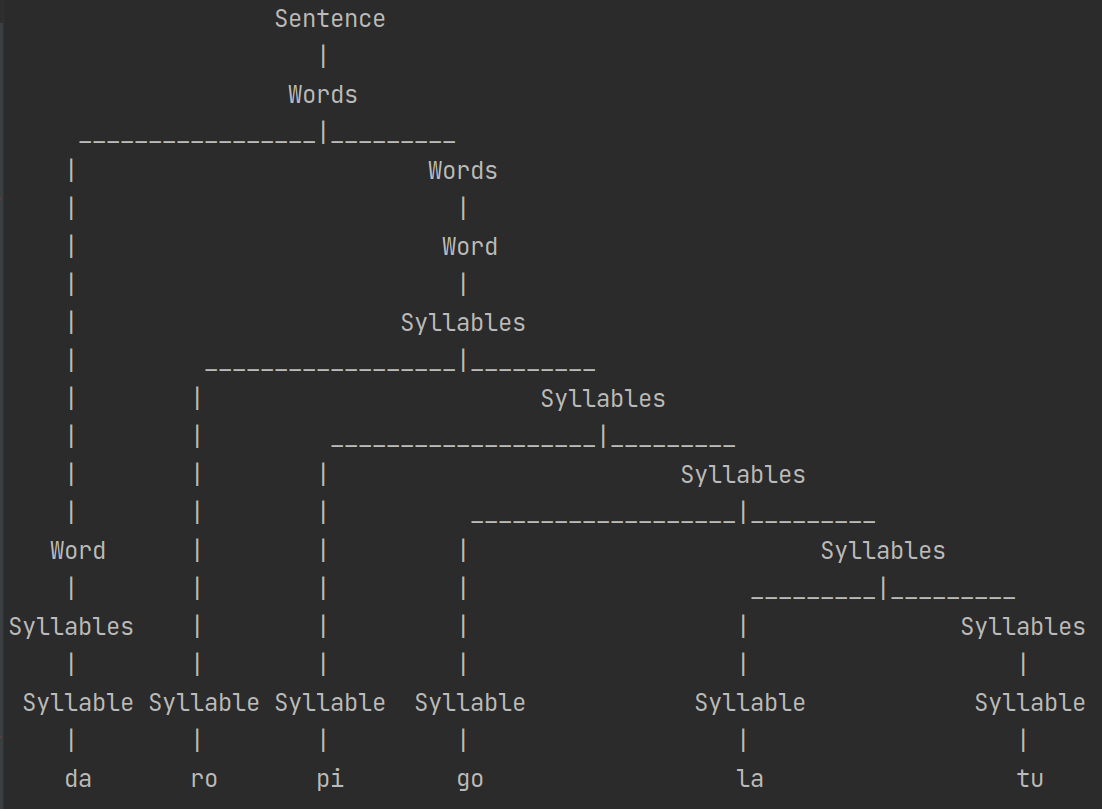
\includegraphics[width=\columnwidth]{figures/sample_bad_tree.png}
  \caption{Sample Parse Tree with Low Probability}~\label{fig:figure2}
\end{figure}

% \begin{figure}
%   \centering
%   \fbox{\rule[-.5cm]{0cm}{4cm}
%   \includegraphics[scale=0.8]{sample_tree.png}
%   \rule[-.5cm]{4cm}{0cm}}
%   \caption{Sample figure caption.}
% \end{figure}


\subsection{Parser Ranking}
We also try four different parsers and do a comparative analysis of the time taken by them to compute all parses of the input `da ro pi go la tu', in an attempt to compare with human reaction times. We receive the following values, as shown in Fig~\ref{fig:figure3}. Saffran et al. gave the infants a much higher threshold of 2 seconds to judge word familiarity.

% \newpage

% \texttt{-------------------------+----------------------------------------------------\\
%   Parser           Beam | Time (secs)   \# Parses   Average P(parse)\\
% -------------------------+----------------------------------------------------\\
%   InsideChartParser    0 |     0.0172         32   0.00000004368648\\
%   RandomChartParser    0 |     0.0371         32   0.00000004368648\\
% UnsortedChartParser    0 |     0.0206         32   0.00000004368648\\
%  LongestChartParser    0 |     0.0170         32   0.00000004368648\\
% -------------------------+----------------------------------------------------\\
%       (All Parses)      |        n/a         32   0.00000000136520
% }

\begin{figure}[h!]
  \centering
  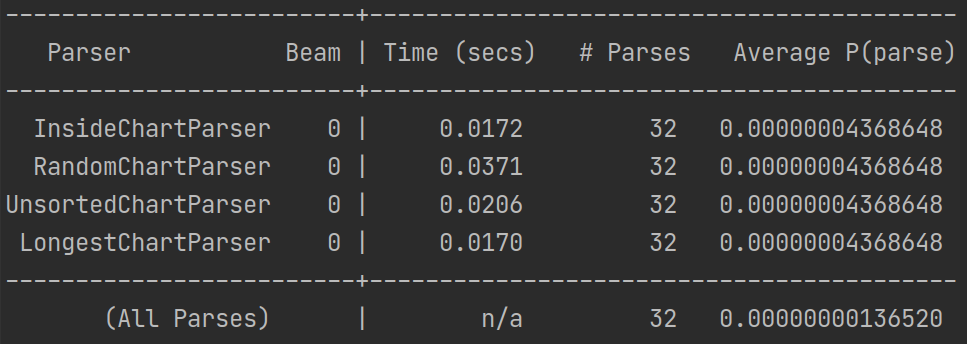
\includegraphics[width=\columnwidth]{figures/parser_times.png}
  \caption{Parser Time Benchmarking}~\label{fig:figure3}
\end{figure}

\vspace{-3mm}
\subsection{Results}
We see that just as Saffran et al. predicted for human infant judgements, for a majority of our randomized experiments, the PCFGs also pick up on a higher transitional probability between two sounds in a word, as compared to two sounds across word boundaries. We thus believe that a probabilistic model can be built to accurately pick up on cues similar to human cognition, while recognising the fact that this method works well only on smaller lexicons and as the number of words increase, the number of rules in a PCFG also increase drastically.

\section{Dynamic Programming with Probabilistic \texttt{n}-gram Modeling}
In addition to the PCFG modeling, we then go on to other probabilistic modeling techniques for word segmentation. We use a model implemented along the lines of Peter Norvig's in the book `Beautiful Data' by \citet{segaran_hammerbacher_2009}.

\subsection{Dataset}
We use Norvig's pre-processed version of the Google Trillion Word Dataset distributed through the Linguistics Data Consortium. This dataset is trimmed of \texttt{n}-grams occurring lower than 40 times, unkified, and sentence demarcations are added. It readily gives us unigram and bigram probabilities, from which we can compute the conditional probabilities as well. A snapshot of the bigram counts data used is in Fig~\ref{fig:figure4}.

\begin{figure}[h!]
  \centering
  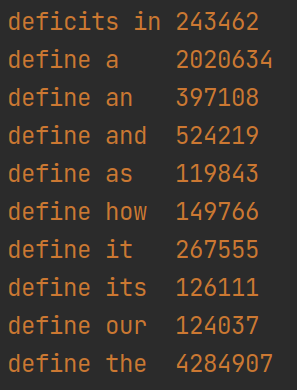
\includegraphics[scale=0.6]{figures/bigram_counts.png}
  \caption{Bigram Counts Dataset Snapshot}~\label{fig:figure4}
\end{figure}
\vspace{-3mm}
\subsection{Modeling and Implementation}
We use two probabilistic models---one based on unigrams and the other on bigrams. We recursively split a stream of text, computing the Naive Bayes probability of the sequence of words thus formed, and use dynamic programming to memoize our computation, preventing us from running into exponential times. The Bayes probability is computed using a probability distribution estimated from the counts in the pre-processed data files, and Laplace additive smoothing is used to estimate the probability of unknown words. We also use surprisal values for the bigram model. Finally, the segmentation with the highest probability, or the lowest surprisal, is chosen as our output segmentation.
\vspace{-1mm}
\subsection{Testing and Results}
\vspace{-1mm}
We create a unit test file, with segmentations of text stream, both straightforward and ambiguous, e.g., `choosespain' can be segmented both as `choose spain' or `chooses pain'. If we believe that humans use statistical inference, then we can assume that the former would be more probable than the latter, based on conditional probability counts of the true. This is a hypothesis we test in our model, and it indeed turns out to be true. A snapshot of our test file is in Fig~\ref{fig:figure5}. Overall, while this model performs well, there remain controversies as to how well such models relate to human cognitive processes.
\vspace{-1mm}
\begin{figure}[h!]
  \centering
  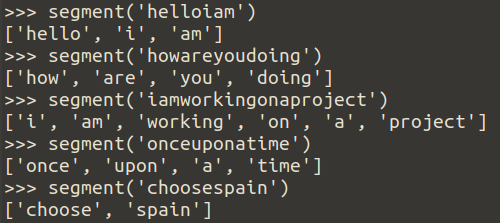
\includegraphics[scale=0.8]{figures/ngram_test_set.png}
  \caption{Test Set Snapshot}~\label{fig:figure5}
\end{figure}

\subsection{Extra: Testing on Japanese}
\vspace{-1mm}
While English employs word spacing, which makes word segmentation from written corpora fairly easy, Japanese does not (and neither do Mandarin, Cantonese and agglutinative languages). This makes Japanese word segmentation a very important problem that every language model based in Japanese needs to face. We trained a bigram model on Wikipedia Japanese data and tested it on Zhang Lang's corpus to come up with the following word segmentation, a snapshot of which is in Fig~\ref{fig:figure6}.

\begin{figure}[h!]
  \centering
  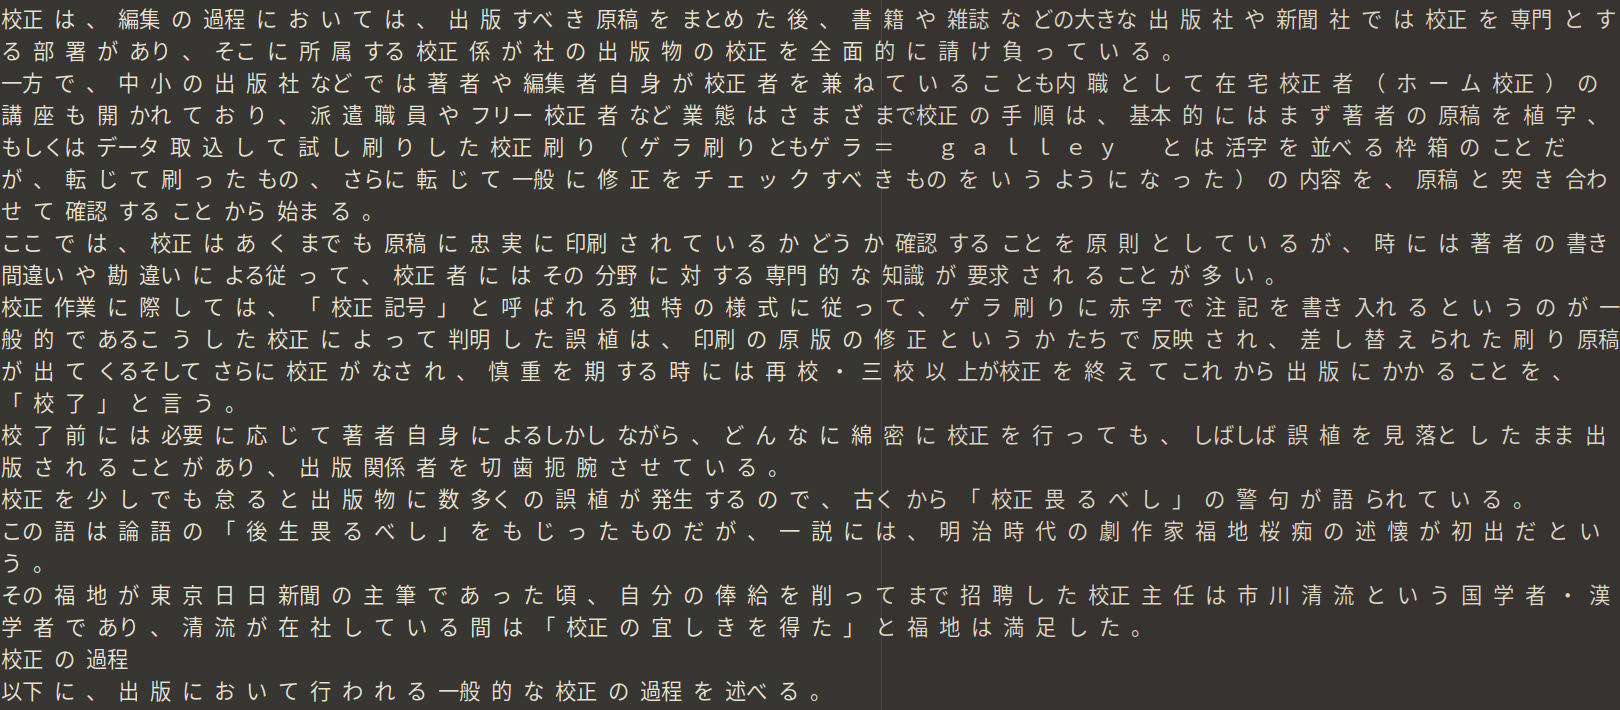
\includegraphics[width=\columnwidth]{figures/Japanese_data.png}
  \caption{Japanese Word Segmentation}~\label{fig:figure6}
%   \vspace{-3mm}
\end{figure}
% \vspace{-10mm}
\section{A Statistical Approach}

We turn our focus to \citet{Venkataraman}'s model, which relies on the probability that a word $w_i$ appears given that some previous words $w_{i-1}, w_{i-2}, \dots$ have already appeared. We estimate the necessary \texttt{n}-grams probabilities in function of other \texttt{n}-grams of lower order and, when we get to \texttt{1}-grams, we back off to the relative frequencies of the phonemes of a given word. The model only focuses on \texttt{1}-grams, \texttt{2}-grams, and \texttt{3}-grams, though this could be extended if necessary. Fig~\ref{fig:fig7} shows a complete description of how we calculate these probabilities. Unlike the focus of the previous models we have seen so far, we will focus on the \textbf{algorithmic level} description of this model.

\begin{figure}[h!]
    \centering
    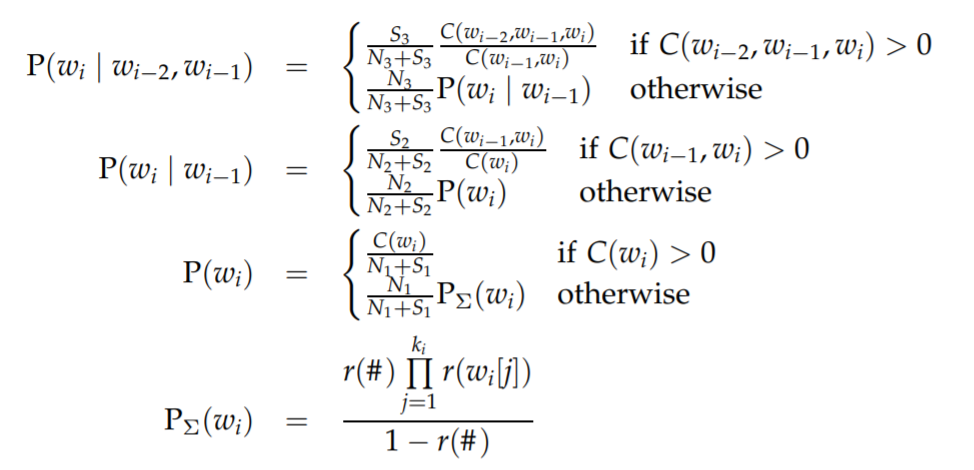
\includegraphics[scale=0.8]{figures/venkataraman_1.PNG}
    \caption{$N_i$ denotes the number of distincts \texttt{i}-grams, $S_i$ is the some of their frequencies, C() is the count function, r() denotes the relative frequency function. Taken from \citet{Venkataraman}}
    \label{fig:fig7}
\end{figure}
% \vspace{-3mm}
\subsection{Dataset}
We use the same dataset as \citet{Brent}, that consists of transcripts made by Bernstein-Ratner (1987) of the CHILDES Database (MacWhinney and Snow 1985). This dataset consists of nine mothers talking freely to their children (13-21 months old), which we hope will give us a good estimate on how children understand a speech stream. Fig~\ref{fig:fig8} shows some examples of this dataset.
\begin{figure}[h!]
    \centering
    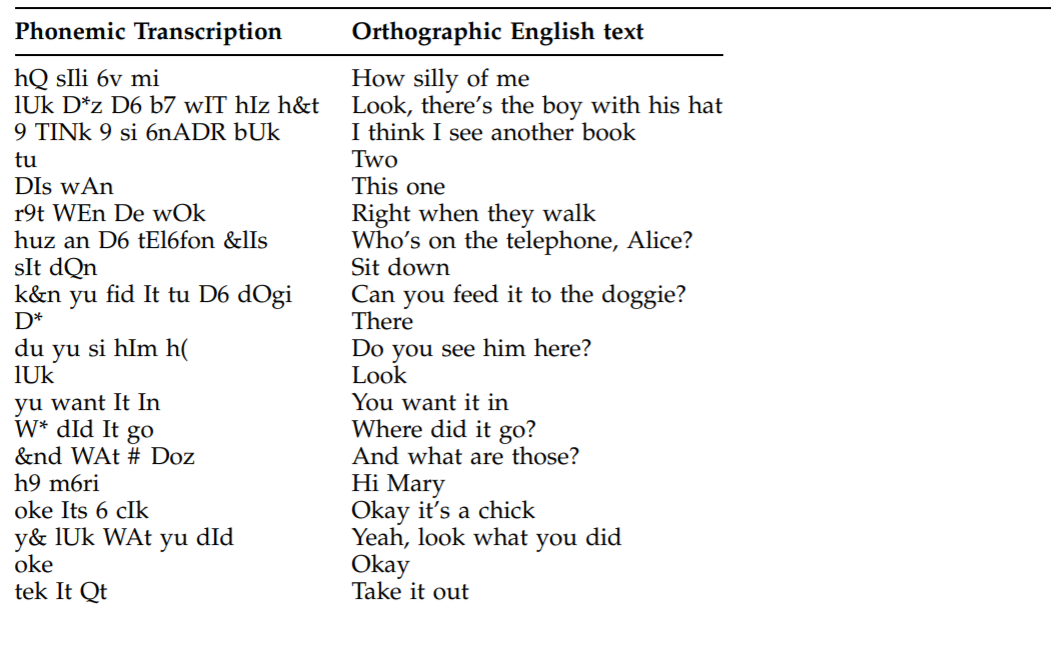
\includegraphics[scale=0.8]{figures/venkataram_corpus_example.PNG}
    \caption{Twenty randomly chosen examples from the input corpus, written with their orthographic transcripts. Taken from \citet{Venkataraman}}
    \label{fig:fig8}
\end{figure}
\subsection{Algorithm}
To find word boundaries in a given utterance, we try to split it at a given place and check what the \textit{score} is. Then we take the lowest score of all the segmentations.  For example, Fig~\ref{fig:fig9} represents what we would do if we were trying to segment the word $s = abcde$

\begin{figure}[h]
    \centering
    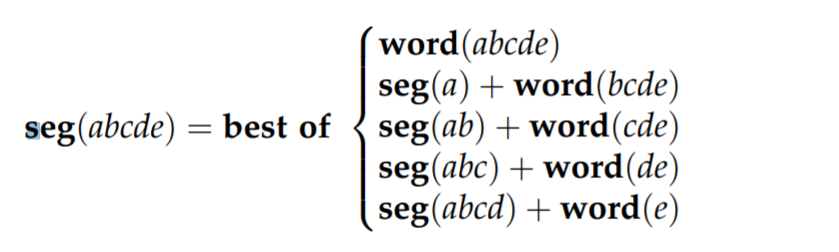
\includegraphics[scale=0.8]{figures/venkataram_seg_example.PNG}
    \caption{Example to segment s = abcde. Taken from \citet{Venkataraman}}
    \label{fig:fig9}
\end{figure}

where \textbf{seg} is our function of interest and \textbf{word} is a way of scoring each word we find. A pseudocode description of that function is shown in Fig~\ref{fig:fig10}.

\begin{figure}[h!]
    \centering
    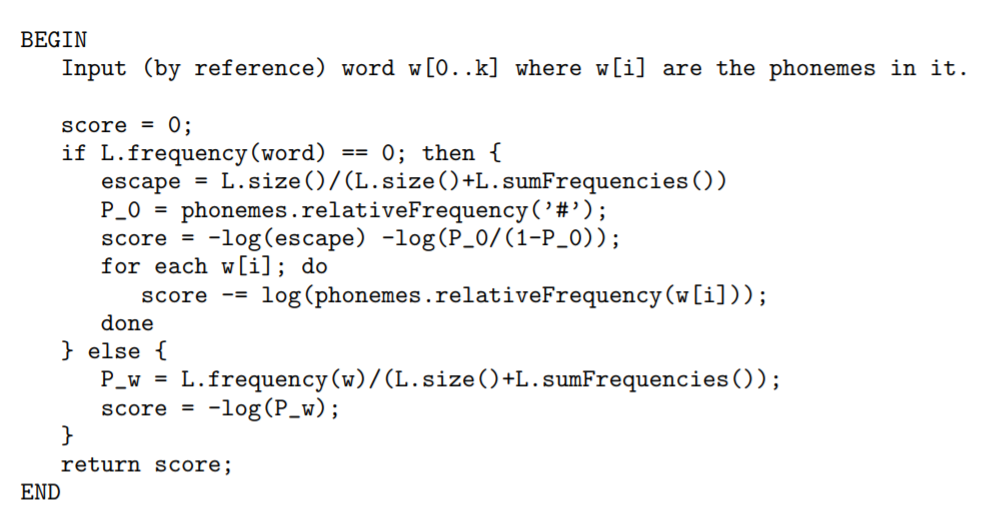
\includegraphics[scale=0.8]{figures/venkataram_evalword.PNG}
    \caption{Description of \texttt{evalWord}. If the word is novel, then the model uses a distribution over the phonemes of the word. Taken from \citet{Venkataraman}}
    \label{fig:fig10}
\end{figure}

\subsection{Results}
In order to avoid any bias the original corpus might have in terms of the order the sentences are presented, we first shuffle all the sentences before processing. Below are shown some examples of the segmentations that this model was able to perform. 
\begin{minted}
[
frame=lines,
framesep=2mm,
baselinestretch=1.2
% fontsize=\footnotesize,
% linenos
]
{python}
    """ 
    For #6n El6f6nt#, the segmentation is 6n El#6f6nt#
    
    For #pUl It Qt kwIk#, the segmentation is pU#l #It #QtkwIk#
    
    For #WAts DIs gel#, the segmentation is WAt#s DI#s gel#
    
    For #WAts D&t#, the segmentation is WAt#s D&t# 
    
    For #WAts DIs#, the segmentation is WAt#s DIs# 
    """
\end{minted}
Even though the algorithm used for this is fairly simple, we can still see a reasonable segmentation for those utterances and thus conclude the usefulness of this method.
\subsection{Model improvement}
In order to obtain a more accurate segmenter, we could try using a larger input corpus (currently it onlye contains 9790 utterances and 33,399 words) and have longer utterances to update our model with more significant data. 

On the other hand, we could change the way that \textbf{evalWord} works when finding novel words. Currently, it focuses on the statistical frequency of the phonemes of the word. We could, for example, have this value be drawn from another probability distribution instead. In Lecture 3, we are told that {\it{A representation of degrees of belief in terms of probability theory is necessary to cohere with common sense}}, which is exactly what we are trying to achieve. As such, we believe that, for example, putting prior probabilities on the types of words our model tries to learn will significantly improve its performance. We could use this technique to prevent the model from picking segmentations that are not phonotactically correct. This is similar in nature to the discussion in class around priors in The Number Game, where we assigned low priors to hypotheses that go against ``common sense".
% \section{Resultle' s and Discussion}
% \section{Model Comparison}
\vspace{-2mm}
\section{Conclusion}
\vspace{-1mm}
In this paper, we have detailed how the computational model based on \citet{Saffran1996}'s infant learning experiment, as well as those based on \citet{segaran_hammerbacher_2009}, and \citet{Venkataraman}
function, how they are implemented, and how they perform on the segmentation task given varying kinds of inputs---whether it be nonce words, English, or Japanese. We have also analysed how these models relate with the human intuition and cognitive experiments. Finally, we discussed some of the advantages and disadvantages of these models, especially in relation to human cognition, as well as ways to improve on the models and directions for future work.
\vspace{-2mm}
\section{Future Work}
\vspace{-1mm}
We wish to extend this work in the future, both along the experimental cognitive science and the computational directions. Our future plans include \begin{itemize}
    \item collecting our own human data for nonce speech streams (similar to Saffran et al.'s) and seeing how our PCFG model compares to human learners
    \item simulating a beginner language learner with PCFGs---one who adjusts the probability in their mental PCFG representation for every new syllable seen, and then investigating into how the rules change (this is something one of us is working on from a phoneme-learning point-of-view on another project and finds really interesting)
    \item extending the probabilistic \texttt{n}-gram word segmentation algorithm to other languages
\end{itemize}

\section{Contribution}
Shinjini has developed, implemented and tested the PCFG model as well as implemented and tested the first probabilistic \texttt{n}-gram model mentioned. She has also written out the corresponding sections in the paper, as well as the Abstract, Motivation and Future Work sections.

Raul has helped in testing of the PCFG model, and has implemented and tested the second statistical model mentioned. He has written out the corresponding sections in the paper, as well as the Introduction and the Conclusion.

% \section{Conclusion}

% NeurIPS requires electronic submissions.  The electronic submission site is
% \begin{center}
%   \url{https://cmt3.research.microsoft.com/NeurIPS2020/}
% \end{center}

% Please read the instructions below carefully and follow them faithfully.

% \subsection{Style}

% Papers to be submitted to NeurIPS 2020 must be prepared according to the
% instructions presented here. Papers may only be up to eight pages long,
% including figures. Additional pages \emph{containing only a section on the broader impact, acknowledgments and/or cited references} are allowed. Papers that exceed eight pages of content will not be reviewed, or in any other way considered for
% presentation at the conference.

% The margins in 2020 are the same as those in 2007, which allow for $\sim$$15\%$
% more words in the paper compared to earlier years.

% Authors are required to use the NeurIPS \LaTeX{} style files obtainable at the
% NeurIPS website as indicated below. Please make sure you use the current files
% and not previous versions. Tweaking the style files may be grounds for
% rejection.

% \subsection{Retrieval of style files}

% The style files for NeurIPS and other conference information are available on
% the World Wide Web at
% \begin{center}
%   \url{http://www.neurips.cc/}
% \end{center}
% The file \verb+neurips_2020.pdf+ contains these instructions and illustrates the
% various formatting requirements your NeurIPS paper must satisfy.

% The only supported style file for NeurIPS 2020 is \verb+neurips_2020.sty+,
% rewritten for \LaTeXe{}.  \textbf{Previous style files for \LaTeX{} 2.09,
%   Microsoft Word, and RTF are no longer supported!}

% The \LaTeX{} style file contains three optional arguments: \verb+final+, which
% creates a camera-ready copy, \verb+preprint+, which creates a preprint for
% submission to, e.g., arXiv, and \verb+nonatbib+, which will not load the
% \verb+natbib+ package for you in case of package clash.

% \paragraph{Preprint option}
% If you wish to post a preprint of your work online, e.g., on arXiv, using the
% NeurIPS style, please use the \verb+preprint+ option. This will create a
% nonanonymized version of your work with the text ``Preprint. Work in progress.''
% in the footer. This version may be distributed as you see fit. Please \textbf{do
%   not} use the \verb+final+ option, which should \textbf{only} be used for
% papers accepted to NeurIPS.

% At submission time, please omit the \verb+final+ and \verb+preprint+
% options. This will anonymize your submission and add line numbers to aid
% review. Please do \emph{not} refer to these line numbers in your paper as they
% will be removed during generation of camera-ready copies.

% The file \verb+neurips_2020.tex+ may be used as a ``shell'' for writing your
% paper. All you have to do is replace the author, title, abstract, and text of
% the paper with your own.

% The formatting instructions contained in these style files are summarized in
% Sections \ref{gen_inst}, \ref{headings}, and \ref{others} below.

% \section{General formatting instructions}
% \label{gen_inst}

% The text must be confined within a rectangle 5.5~inches (33~picas) wide and
% 9~inches (54~picas) long. The left margin is 1.5~inch (9~picas).  Use 10~point
% type with a vertical spacing (leading) of 11~points.  Times New Roman is the
% preferred typeface throughout, and will be selected for you by default.
% Paragraphs are separated by \nicefrac{1}{2}~line space (5.5 points), with no
% indentation.

% The paper title should be 17~point, initial caps/lower case, bold, centered
% between two horizontal rules. The top rule should be 4~points thick and the
% bottom rule should be 1~point thick. Allow \nicefrac{1}{4}~inch space above and
% below the title to rules. All pages should start at 1~inch (6~picas) from the
% top of the page.

% For the final version, authors' names are set in boldface, and each name is
% centered above the corresponding address. The lead author's name is to be listed
% first (left-most), and the co-authors' names (if different address) are set to
% follow. If there is only one co-author, list both author and co-author side by
% side.

% Please pay special attention to the instructions in Section \ref{others}
% regarding figures, tables, acknowledgments, and references.

% \section{Headings: first level}
% \label{headings}

% All headings should be lower case (except for first word and proper nouns),
% flush left, and bold.

% First-level headings should be in 12-point type.

% \subsection{Headings: second level}

% Second-level headings should be in 10-point type.

% \subsubsection{Headings: third level}

% Third-level headings should be in 10-point type.

% \paragraph{Paragraphs}

% There is also a \verb+\paragraph+ command available, which sets the heading in
% bold, flush left, and inline with the text, with the heading followed by 1\,em
% of space.

% \section{Citations, figures, tables, references}
% \label{others}

% These instructions apply to everyone.

% \subsection{Citations within the text}

% The \verb+natbib+ package will be loaded for you by default.  Citations may be
% author/year or numeric, as long as you maintain internal consistency.  As to the
% format of the references themselves, any style is acceptable as long as it is
% used consistently.

% The documentation for \verb+natbib+ may be found at
% \begin{center}
%   \url{http://mirrors.ctan.org/macros/latex/contrib/natbib/natnotes.pdf}
% \end{center}
% Of note is the command \verb+\citet+, which produces citations appropriate for
% use in inline text.  For example,
% \begin{verbatim}
%   \citet{hasselmo} investigated\dots
% \end{verbatim}
% produces
% \begin{quote}
%   Hasselmo, et al.\ (1995) investigated\dots
% \end{quote}

% If you wish to load the \verb+natbib+ package with options, you may add the
% following before loading the \verb+neurips_2020+ package:
% \begin{verbatim}
%   \PassOptionsToPackage{options}{natbib}
% \end{verbatim}

% If \verb+natbib+ clashes with another package you load, you can add the optional
% argument \verb+nonatbib+ when loading the style file:
% \begin{verbatim}
%   \usepackage[nonatbib]{neurips_2020}
% \end{verbatim}

% As submission is double blind, refer to your own published work in the third
% person. That is, use ``In the previous work of Jones et al.\ [4],'' not ``In our
% previous work [4].'' If you cite your other papers that are not widely available
% (e.g., a journal paper under review), use anonymous author names in the
% citation, e.g., an author of the form ``A.\ Anonymous.''

% \subsection{Footnotes}

% Footnotes should be used sparingly.  If you do require a footnote, indicate
% footnotes with a number\footnote{Sample of the first footnote.} in the
% text. Place the footnotes at the bottom of the page on which they appear.
% Precede the footnote with a horizontal rule of 2~inches (12~picas).

% Note that footnotes are properly typeset \emph{after} punctuation
% marks.\footnote{As in this example.}

% \subsection{Figures}

% \begin{figure}
%   \centering
%   \fbox{\rule[-.5cm]{0cm}{4cm} \rule[-.5cm]{4cm}{0cm}}
%   \caption{Sample figure caption.}
% \end{figure}

% All artwork must be neat, clean, and legible. Lines should be dark enough for
% purposes of reproduction. The figure number and caption always appear after the
% figure. Place one line space before the figure caption and one line space after
% the figure. The figure caption should be lower case (except for first word and
% proper nouns); figures are numbered consecutively.

% You may use color figures.  However, it is best for the figure captions and the
% paper body to be legible if the paper is printed in either black/white or in
% color.

% \subsection{Tables}

% All tables must be centered, neat, clean and legible.  The table number and
% title always appear before the table.  See Table~\ref{sample-table}.

% Place one line space before the table title, one line space after the
% table title, and one line space after the table. The table title must
% be lower case (except for first word and proper nouns); tables are
% numbered consecutively.

% Note that publication-quality tables \emph{do not contain vertical rules.} We
% strongly suggest the use of the \verb+booktabs+ package, which allows for
% typesetting high-quality, professional tables:
% \begin{center}
%   \url{https://www.ctan.org/pkg/booktabs}
% \end{center}
% This package was used to typeset Table~\ref{sample-table}.

% \begin{table}
%   \caption{Sample table title}
%   \label{sample-table}
%   \centering
%   \begin{tabular}{lll}
%     \toprule
%     \multicolumn{2}{c}{Part}                   \\
%     \cmidrule(r){1-2}
%     Name     & Description     & Size ($\mu$m) \\
%     \midrule
%     Dendrite & Input terminal  & $\sim$100     \\
%     Axon     & Output terminal & $\sim$10      \\
%     Soma     & Cell body       & up to $10^6$  \\
%     \bottomrule
%   \end{tabular}
% \end{table}

% \section{Final instructions}

% Do not change any aspects of the formatting parameters in the style files.  In
% particular, do not modify the width or length of the rectangle the text should
% fit into, and do not change font sizes (except perhaps in the
% \textbf{References} section; see below). Please note that pages should be
% numbered.

% \section{Preparing PDF files}

% Please prepare submission files with paper size ``US Letter,'' and not, for
% example, ``A4.''

% Fonts were the main cause of problems in the past years. Your PDF file must only
% contain Type 1 or Embedded TrueType fonts. Here are a few instructions to
% achieve this.

% \begin{itemize}

% \item You should directly generate PDF files using \verb+pdflatex+.

% \item You can check which fonts a PDF files uses.  In Acrobat Reader, select the
%   menu Files$>$Document Properties$>$Fonts and select Show All Fonts. You can
%   also use the program \verb+pdffonts+ which comes with \verb+xpdf+ and is
%   available out-of-the-box on most Linux machines.

% \item The IEEE has recommendations for generating PDF files whose fonts are also
%   acceptable for NeurIPS. Please see
%   \url{http://www.emfield.org/icuwb2010/downloads/IEEE-PDF-SpecV32.pdf}

% \item \verb+xfig+ "patterned" shapes are implemented with bitmap fonts.  Use
%   "solid" shapes instead.

% \item The \verb+\bbold+ package almost always uses bitmap fonts.  You should use
%   the equivalent AMS Fonts:
% \begin{verbatim}
%   \usepackage{amsfonts}
% \end{verbatim}
% followed by, e.g., \verb+\mathbb{R}+, \verb+\mathbb{N}+, or \verb+\mathbb{C}+
% for $\mathbb{R}$, $\mathbb{N}$ or $\mathbb{C}$.  You can also use the following
% workaround for reals, natural and complex:
% \begin{verbatim}
%   \newcommand{\RR}{I\!\!R} %real numbers
%   \newcommand{\Nat}{I\!\!N} %natural numbers
%   \newcommand{\CC}{I\!\!\!\!C} %complex numbers
% \end{verbatim}
% Note that \verb+amsfonts+ is automatically loaded by the \verb+amssymb+ package.

% \end{itemize}

% If your file contains type 3 fonts or non embedded TrueType fonts, we will ask
% you to fix it.

% \subsection{Margins in \LaTeX{}}

% Most of the margin problems come from figures positioned by hand using
% \verb+\special+ or other commands. We suggest using the command
% \verb+\includegraphics+ from the \verb+graphicx+ package. Always specify the
% figure width as a multiple of the line width as in the example below:
% \begin{verbatim}
%   \usepackage[pdftex]{graphicx} ...
%   \includegraphics[width=0.8\linewidth]{myfile.pdf}
% \end{verbatim}
% See Section 4.4 in the graphics bundle documentation
% (\url{http://mirrors.ctan.org/macros/latex/required/graphics/grfguide.pdf})

% A number of width problems arise when \LaTeX{} cannot properly hyphenate a
% line. Please give LaTeX hyphenation hints using the \verb+\-+ command when
% necessary.


% \section*{Broader Impact}

% Authors are required to include a statement of the broader impact of their work, including its ethical aspects and future societal consequences. 
% Authors should discuss both positive and negative outcomes, if any. For instance, authors should discuss a) 
% who may benefit from this research, b) who may be put at disadvantage from this research, c) what are the consequences of failure of the system, and d) whether the task/method leverages
% biases in the data. If authors believe this is not applicable to them, authors can simply state this.

% Use unnumbered first level headings for this section, which should go at the end of the paper. {\bf Note that this section does not count towards the eight pages of content that are allowed.}

% \begin{ack}
% Use unnumbered first level headings for the acknowledgments. All acknowledgments
% go at the end of the paper before the list of references. Moreover, you are required to declare 
% funding (financial activities supporting the submitted work) and competing interests (related financial activities outside the submitted work). 
% More information about this disclosure can be found at: \url{https://neurips.cc/Conferences/2020/PaperInformation/FundingDisclosure}.


% Do {\bf not} include this section in the anonymized submission, only in the final paper. You can use the \texttt{ack} environment provided in the style file to autmoatically hide this section in the anonymized submission.
% \end{ack}

% \section*{References}

% References follow the acknowledgments. Use unnumbered first-level heading for
% the references. Any choice of citation style is acceptable as long as you are
% consistent. It is permissible to reduce the font size to \verb+small+ (9 point)
% when listing the references.
% {\bf Note that the Reference section does not count towards the eight pages of content that are allowed.}
% \medskip

% \small

% [1] Alexander, J.A.\ \& Mozer, M.C.\ (1995) Template-based algorithms for
% connectionist rule extraction. In G.\ Tesauro, D.S.\ Touretzky and T.K.\ Leen
% (eds.), {\it Advances in Neural Information Processing Systems 7},
% pp.\ 609--616. Cambridge, MA: MIT Press.

% [2] Bower, J.M.\ \& Beeman, D.\ (1995) {\it The Book of GENESIS: Exploring
%   Realistic Neural Models with the GEneral NEural SImulation System.}  New York:
% TELOS/Springer--Verlag.

% [3] Hasselmo, M.E., Schnell, E.\ \& Barkai, E.\ (1995) Dynamics of learning and
% recall at excitatory recurrent synapses and cholinergic modulation in rat
% hippocampal region CA3. {\it Journal of Neuroscience} {\bf 15}(7):5249-5262.

\bibliography{bibliography}


\end{document}
